%% TODO
%% 1. illustrating figures
%% 2. add section on MST in DAGs
%%
\documentclass{beamer}
\setbeamertemplate{footline}[frame number]

\usepackage[utf8x]{inputenc}
\usepackage[brazil,british]{babel}
\usetheme{default} 
\usecolortheme{beaver}
\newtranslation[to=brazil]{Theorem}{Teorema}
\newtranslation[to=brazil]{Definition}{Definição}
\newtranslation[to=brazil]{Example}{Exemplo}
\newtranslation[to=brazil]{Problem}{Exercício}
\newtranslation[to=brazil]{Solution}{Resolução}
\logo{
\includegraphics[width=1cm]{../img/logo-ppgsc-icon-text.png}}

\usepackage{graphicx}
\usepackage{clrscode3e}
\usepackage{hyperref}

\usepackage{pgf}
\usepackage{tikz}
\newcommand{\assert}[1]{\textcolor{blue}{#1}}



\title{Aula 27: Programação dinâmica}
\author{David Déharbe \\
  Programa de Pós-graduação em Sistemas e Computação \\
  Universidade Federal do Rio Grande do Norte \\
  Centro de Ciências Exatas e da Terra \\
  Departamento de Informática e Matemática Aplicada}
\date{25 de maio de 2015}

\begin{document}
\selectlanguage{brazil}

%%%%% SLIDE %%%%%

\begin{frame}
  \titlepage
\end{frame}

\begin{frame}
  \frametitle{Plano}

  \tableofcontents
Referência: Cormen, cap 16.
\end{frame}

\section{Introdução}

%%%%% SLIDE %%%%%

\begin{frame}
\frametitle{Introdução}

\begin{itemize}
\item qual forma ótima de escolher $N$ objetos, cada um com peso $w_1, \ldots,
  w_n$, e valores $v_1, \ldots v_n$, para levar em uma mala de até $K$
  kilogramas?
\item qual a maior subsequência comum a duas sequências?
\item qual a quantidade mínima de edições (adição/remoção/troca) para passar de uma palavra à outra?
\item qual a ordem ótima para multiplicar $N$ matrizes $A_1, \ldots A_N$?
\item como escolher valores dentre de um conjunto de tal forma que a soma deles seja nula?
\end{itemize}
\pause
\alert{programação dinâmica!}

\end{frame}

%%%%% SLIDE %%%%%

\begin{frame}
\frametitle{Origem}

\begin{itemize}
\item 1940--1950 Richard Bellman
\begin{itemize}
\item o mesmo do algoritmo de Bellman-Ford
\end{itemize}
\item contexto: resolução de problemas envolvendo tomadas de decisões sucessivas
\item \textit{dynamic programming}: construção dinâmica de uma programação.
\end{itemize}

\end{frame}

\section{Princípios gerais}

%%%%% SLIDE %%%%%

\begin{frame}
\frametitle{Princípios}

\begin{itemize}
\item decomposição: a solução para uma instância $I$ pode ser expressa a partir
  das soluções para instâncias menores $I_1, \ldots I_n$ derivadas de $I$
\item aplicar sucessivamente esta decomposição leva a ter que solucionar várias
  vezes o mesmo sub-problema. \alert{sub-problemas sobrepostos}
\item a melhor solução para $I$ pode ser obtida a partir das melhores
  soluções para $I_1, \ldots I_n$. \alert{sub-estrutura ótima}
\end{itemize}

\end{frame}

\section{Exemplo introdutório}

\begin{frame}

\frametitle{Exemplo 1}

\begin{eqnarray*}
\id{fib}(0) & = & 0 \\
\id{fib}(1) & = & 1 \\
\id{fib}(n) & = & \id{fib}(n-1) + \id{fib}(n-2) \text{para $n \ge 2$}
\end{eqnarray*}

\begin{enumerate}
\item sub-estrutura ótima: não há otimização
\item sub-problemas sobrepostos: não calcular duas vezes o mesmo resultado
\end{enumerate}

\begin{itemize}
\item recursão + memorização das soluções dos sub-problemas
\end{itemize}

\end{frame}

\begin{frame}

\frametitle{Exemplo 1}
\framesubtitle{Resolução computational}

\begin{itemize}
\item abordagem ascendente
\begin{itemize}
\item iniciar dos sub-problemas mais simples possíveis
\item calcular sub-problemas cada vez maiores
\item $\id{fib}(0), \id{fib}(1), \id{fib}(2), \ldots , \id{fib}(n)$.
\end{itemize}
\item abordagem descendente
\begin{itemize}
\item quebrar o problema em sub-problemas mais simples
\item solucionar os sub-problemas gerados
\item $\id{fib}(n), \id{fib}(n-1), \id{fib}(n-2), \id{fib}(n-3) \ldots , \id{fib}(0)$.
\item \alert{memorizar} as soluções já calculadas
\end{itemize}
\end{itemize}

\end{frame}

\begin{frame}

\frametitle{Exercício}

\begin{itemize}
\item Escrever um algoritmo para calcular $\id{fib}(n)$ utilizando a abordagem
ascendente
\item Escrever um algoritmo para calcular $\id{fib}(n)$ utilizando a abordagem
descendente
\end{itemize}

\end{frame}

\section{Exemplo intermediário}

\begin{frame}
\frametitle{Exemplo: um problema de tabuleiro}

\begin{itemize}
\item É dado um tabuleiro $N \times M$ tal que há um custo $C_{i, j}$ associado
  à sub-divisão da linha $i$ e da coluna $j$.

\item Projetar um algoritmo que determina o menor custo para atravessar o
  tabuleiro da primeira até a última linha?

\end{itemize}

\end{frame}

\begin{frame}
\frametitle{Análise do problema}

\begin{itemize}

\item Se $M=1$, há um único caminho possível

\item Se $M \ge 2$, quantos caminhos são possíveis?

\begin{tabular}{|c|c|c|c|c|c|c|c|c|}
\hline
1 & 1 & 1 & 1 & 1 & 1 & 1 & 1 & 1 \\
\hline
2 & 3 & 3 & 3 & 3 & 3 & 3 & 3 & 2 \\
\hline
5 & 8 & 9 & 9 & 9 & 9 & 9 & 8 & 2 \\
\hline
13 & 22 & 26 & 27 & 27 & 27 & 26 & 22 & 13 \\
\hline
\end{tabular}

\item para cada sub-divisão: $\Omega(2^{N-1})$ e $O(3^{N-1})$ caminhos

\item total: $\Omega(M \cdot 2^{N-1})$ e $O(M \cdot 3^{N-1})$ caminhos

\item exponencial

\item muitos caminhos possuem trechos comuns 

\begin{itemize}

\item \alert{sub-problemas sobrepostos}

\end{itemize}

\end{itemize}

\end{frame}

\begin{frame}
\frametitle{Análise do problema}

\begin{itemize}
\item Como calcular o menor custo para uma sub-divisão?

\item $P_{i, j}$: custo da sub-divisão $(i, j)$

\item $C_{i, j}$: menor custo para chegar à divisão $(i, j)$

\item $i > 1$, sub-divisão fora da borda:
\begin{center}
\begin{tabular}{|c|c|c|}
\hline
$C_{i-1, j-1}$ & $C_{i-1, j}$ & $C_{i-1, j+1}$ \\
\hline
              & $P_{i, j}$ &  \\
\hline
\end{tabular}
\end{center}
\item $C_{i, j} = P_{i, j} + \min \{ C_{i-1, j-1}, C_{i-1, j}, C_{i-1, j+1} \}$

\item $i > 1$, sub-divisão na borda:
\begin{center}
\begin{tabular}{ccc}
\begin{tabular}{|c|c|}
\hline
$C_{i-1, 1}$ & $C_{i-1, 2}$ \\
\hline
$P_{i, 1}$ &  \\
\hline
\end{tabular}
& ou &
\begin{tabular}{|c|c|}
\hline
$C_{i-1, M-1}$ & $C_{i-1, M}$ \\
\hline
              & $P_{i, M}$ \\
\hline
\end{tabular}
\end{tabular}
\end{center}
\item $C_{i, 1} = P_{i, 1} + \min \{ C_{i-1, 1}, C_{i-1, 2}$
ou $C_{i, M} = P_{i, M-1} + \min \{ C_{i-1, 1}, C_{i-1, M}$

\begin{itemize}

\item \alert{sub-estrutura ótima}

\end{itemize}

\end{itemize}

\end{frame}

\begin{frame}

\frametitle{Algoritmo}

\begin{itemize}
\item Queremos calcular $C[i, j]$ para cada $i, j$.
\item Concluído este cálculo, basta determinar o menor valor 
entre os $C[N, j]$.
\end{itemize}
\begin{small}
\begin{codebox}
\li \For $j = 1 \To M$
\li \Do $C[1, j] \gets P[1, j]$
    \End
\li \For $i = 2 \To N$
\li \Do $C[i, 1] \gets P[i, 1] + \min \{ C[i-1, 1], C[i-1, 2] \}$
\li   $C[i, M] \gets P[i, M] + \min \{ C[i-1, M-1], C[i-1, M] \}$
\li   \For $j = 2 \To M-1$
\li   \Do $C[i, j] \gets P[i, j] + \min \{ C[i-1, j-1], C[i-1, j], C[i-1, j+1] \}$
      \End
    \End
\li $\id{res} \gets C[N, 1]$
\li \For $j = 2 \To N$
\li \Do \If $C[N, j] < \id{res}$
\li    \Then $\id{res} \gets C[N, j]$
       \End
    \End
\li \Return $\id{res}$
\end{codebox}
\end{small}
\end{frame}

\begin{frame}

\frametitle{Algoritmo}

\begin{small}
\begin{codebox}
\li \For $j = 1 \To M$ \only<2>{\assert{\Comment $\Theta(M)$}}
\li \Do $C[1, j] \gets P[1, j]$
    \End
\li \For $i = 2 \To N$  \only<2>{\assert{\Comment $\Theta(N)$ repetições}}
\li \Do $C[i, 1] \gets P[i, 1] + \min \{ C[i-1, 1], C[i-1, 2] \}$
\li   $C[i, M] \gets P[i, M] + \min \{ C[i-1, M-1], C[i-1, M] \}$
\li   \For $j = 2 \To M-1$  \only<2>{\assert{\Comment $\Theta(M)$ repetições}}
\li   \Do $C[i, j] \gets P[i, j] + \min \{ C[i-1, j-1], C[i-1, j], C[i-1, j+1] \}$
      \End
    \End
\li $\id{res} \gets C[N, 1]$
\li \For $j = 2 \To N$
\li \Do \If $C[N, j] < \id{res}$
\li    \Then $\id{res} \gets C[N, j]$
       \End
    \End
\li \Return $\id{res}$
\end{codebox}
\end{small}

Complexidade? \pause \alert{$\Theta(N M)$}
\end{frame}

\begin{frame}
\frametitle{Exercício}

\begin{enumerate}
\item Adapte o algoritmo anterior para imprimir o caminho menos custoso
para atravessar o tabuleiro.
\end{enumerate}
\end{frame}

\section{Exemplo avançado}

\begin{frame}
\frametitle{Exemplo: o problema da multiplicação de matrizes}

\begin{itemize}
\item É dada uma sequência de matrizes de tamanho $L_1 \times C_1$, $L_2 \times
  C_2, \ldots L_n \times C_n$, tal que $L_i = C_{i+1}$, para $1 \le i < n$.

\begin{itemize}
\item exemplo: $A_1: 10 \times 100, A_2: 100 \times 5, A_3: 5 \times 50$
\item $(A_1 \cdot A_2) \cdot A_3$: $10 \cdot 100 \cdot 5 + 10 \cdot 5 \cdot 50 = 7.500$
\item $A_1 \cdot (A_2 \cdot A_3)$: $100 \cdot 5 \cdot 50 + 10 \cdot 100 \cdot 50 = 75.000$
\end{itemize}
\item Projetar um algoritmo que determina a ordem ótima de realizar as
  multiplicações (aquela que minimiza o número de operações entre elementos de
  matrizes).
\item Notação: $A_i$ tem dimensão $p_{i-1} \times p_i$.
\end{itemize}
\end{frame}

\begin{frame}
\frametitle{Análise do problema}

\begin{itemize}
\item Para $n$ matrizes: quantas maneiras existem de calcular o produto delas?
\item $N$ matrizes podem ser divididas de $n-1$ formas diferentes:
$A_1$ e $(A_2 \ldots A_n)$, $(A_1, A_2)$ e $(A_3 \ldots A_n)$, etc.
\item Seja $\pi(n)$ o número de maneiras que podemos calcular o produto de $N$ matrizes.
$$
  \begin{array}[t]{rcl}
    \pi(1) & = & 1 \\
    \pi(n) & = & \pi(1) \cdot \pi(n-1) + \pi(2) \cdot \pi(n-2) + \cdots + \pi(n-1) \cdot \pi(1) \\
    & = & \sum_{k=1}^{n-1} \pi(k) \cdot \pi(n-k) \\
    & = & \frac{1}{n}\left( \begin{array}{c} 2n-2 \\ n-1 \end{array} \right) \\
    & \in & \Omega(4^n / n^{3/2})
  \end{array}
$$
\item crescimento \alert{exponencial}
\end{itemize}

\end{frame}

\begin{frame}

\frametitle{Análise da estrutura do problema}

\begin{itemize}
\item Seja $A_1, \ldots A_n$ as matrizes a multiplicar.
\item Seja $A_{i \twodots j}$ o resultado da multiplicação de $A_i \ldots A_j$
\item Um agrupamento ótimo para $A_1 \ldots A_n$ divide em dois grupos
$A_1 \ldots A_k$ e $A_{k+1} \ldots A_n$.
\item O custo do agrupamento ótimo é o custo de calcular de forma ótima
$A_{1 \twodots k}$ e $A_{k+1 \twodots n}$, mais o custo de multiplicar essas
duas matrizes.
\item Um agrupamento ótimo para calcular $A_{1 \twodots n}$ deve incluir 
agrupamentos ótimos para calcular $A_{1 \twodots k}$ e $A_{k+1 \twodots n}$.
\item e \alert{sub-estrutura ótima}
\end{itemize}

\end{frame}


\begin{frame}

\frametitle{Análise dos sub-problemas}

\begin{itemize}
\item sub-problemas: qual o custo mínimo para calcular $A_i \ldots A_j$, onde $1 \le i \le j \le n$?
\item seja $m[i, j]$ este custo
\item queremos calcular $m[1, n]$
\item caso de base: $i = j$
\begin{itemize}
\item nenhuma operação: $m[i, i] = 0$, para $1 \le i \le n$
\end{itemize}
\item caso geral:
\begin{itemize}
\item se dividir em $k$: $m[i, j] = m[i, k] + m[k, j] + p_{i-1}p_kp_j$.
\item logo $m[i, j] = \min \{ m[i, j] = m[i, k] + m[k, j] + p_{i-1}p_kp_j \cdot i \le k < j \}$ se $i < j$
\end{itemize}
\end{itemize}

\end{frame}

\begin{frame}

\frametitle{Análise dos sub-problemas}

\begin{itemize}
\item sub-problemas: qual índice $k$, tal que $i \le k < $, dividir $A_i \ldots A_j$, em $A_{i \twodots k}$ e $A_{k+1 \twodots j}$, onde $1 \le i \le j \le n$?
\item seja $s[i, j]$ este índice
\item $s[i, j]$ é o índice que minimiza $m[i, k] + m[k, j] + p_{i-1}p_kp_j$.
\item há $\Theta(n^2)$ sub-problemas no total
\item um cálculo recursivo descendente necessita solucionar
repetidas vezes o mesmo problema
\item \alert{sub-problemas sobrepostos}
\item abordagem ascendente: cálculo de $m[i, j]$, $s[i, j]$ após ter
  calculado os sub-problemas contidos
\end{itemize}

\end{frame}

\begin{frame}

\frametitle{Algoritmo}

\begin{codebox}
\li $n \gets \attrib{p}{length} - 1$
\li \For $i = 1$ \To $n$
\li   \Do $m[i, i] \gets 0$
    \End
\li \For $l \gets 2$ \To $n$
\li \Do \For $i \gets 1$ \To $n-l+1$
\li   \Do $j \gets i+l-1$
\li     $m[i, j] \gets \infty$
\li     \For $k \gets 1$ \To $j-1$
\li     \Do $q \gets m[i, k]+m[k+1, j]+p_{i-1}p_kp_j$
\li       \If $q < m[i, j]$
\li       \Then $m[i, j] \gets q$
\li         $s[i, j] \gets k$
          \End
        \End
      \End
    \End
\li \Return $m$ and $s$
\end{codebox}

\end{frame}

\begin{frame}

\frametitle{Algoritmo}
\frametitle{Ilustração}

\begin{tabular}{c|c}
matriz & dimensão \\
\hline
$A_1$ & $ 30 \times 35$ \\
$A_2$ & $ 35 \times 15$ \\
$A_3$ & $ 15 \times 5$ \\
$A_4$ & $ 5 \times 10$ \\
$A_5$ & $ 10 \times 20$ \\
$A_6$ & $ 20 \times 25$
\end{tabular}

\end{frame}

\begin{frame}

\frametitle{Algoritmo}

{ \center \alert{Complexidade?}}

\begin{codebox}
\li $n \gets \attrib{p}{length} - 1$
\li \For $i = 1$ \To $n$
\li   \Do $m[i, i] \gets 0$
    \End
\li \For $l \gets 2$ \To $n$
\li \Do \For $i \gets 1$ \To $n-l+1$
\li   \Do $j \gets i+l-1$
\li     $m[i, j] \gets \infty$
\li     \For $k \gets 1$ \To $j-1$
\li     \Do $q \gets m[i, k]+m[k+1, j]+p_{i-1}p_kp_j$
\li       \If $q < m[i, j]$
\li       \Then $m[i, j] \gets q$
\li         $s[i, j] \gets k$
          \End
        \End
      \End
    \End
\li \Return $m$ and $s$
\end{codebox}
\pause
\alert{$\Theta(n^3)$}
\end{frame}

\begin{frame}
\frametitle{Concluindo: multiplicando matrizes de forma ótima}

\begin{codebox}
\Procname{$\proc{Matrix-Product+}(A, s, i, j)$}
\li \If $j > i$
\li \Then $X \gets \proc{Matrix-Product+}(A, s, i, s[i, j])$
\li    $Y \gets \proc{Matrix-Product+}(A, s, s[i, j]+1, j)$
\li    \Return $\proc{Matrix-Multiply}(X, Y)$
\li \Else \Return $A_i$
    \End
\end{codebox}

\end{frame}

\section{Exercícios}

\begin{frame}

\frametitle{Menor caminho entre duas arestas}

\begin{center}
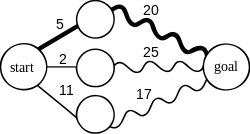
\includegraphics{img/Shortest-path-optimal-substructure.png}
\end{center}

\begin{enumerate}
\item sub-estrutura ótima: em um grafo conectado com pesos, a menor distância de
  $u$ até $v$ pode ser calculada a partir da menor distância dos vértices
  adjacentes a $u$ até $v$.
\item sub-problemas sobrepostos: não calcular duas vezes o mesmo resultado
\end{enumerate}
\begin{itemize}
\item recursão + memorização das soluções dos sub-problemas
\end{itemize}

\end{frame}

\begin{frame}

\frametitle{Exercício}

\begin{enumerate}
\item Escrever um algoritmo para calcular o menor caminho de $u$ até $v$
  utilizando a abordagem ascendente
\item Escrever um algoritmo para calcular o menor caminho de $u$ até $v$
  utilizando a abordagem descendente
\end{enumerate}

\end{frame}

\begin{frame}
\frametitle{Sub-conjunto de soma nula}

\begin{itemize}
\item É dada um conjunto de inteiros $\{v_1, v_2, \ldots v_n\}$.

\item Projetar um algoritmo que determina se existe um sub-conjunto tal que a
  soma dos elementos é nula.
\end{itemize}

\end{frame}

\begin{frame}
\frametitle{Elementos de resposta}

\begin{itemize}
\item Quantos sub-conjuntos de $S = \{v_1, v_2, \ldots v_n\}$?
\item Seja $N$ a soma dos números negativos de $S$
\item Seja $P$ a soma dos números positivos de $S$
\item Seja $Q(i, s)$ verdadeiro sse existe um sub-conjunto de 
$\{v_1, v_2, \ldots v_i\}$ de soma $s$.
\item Representar $Q$ por uma matriz $N+P+1 \times n$
\item Calcular $Q(n, 0)$ soluciona o problema desejado
\item Temos que 
\begin{itemize}
\item $Q(1, s) \leftrightarrow v_1 = s$
\item para $i > 1$: $Q(i, s) \Leftrightarrow 
  \begin{array}[t]{rlr}
         & Q(i-1, s) & \text{$v_i$ não é somado} \\
    \lor & Q(i-1, s-v_i) & \text{$v_i$ é somado} \\
    \lor & s = x_i & \text{a soma é apenas $v_i$}
  \end{array}$
\end{itemize}
\end{itemize}

\end{frame}

\begin{frame}
\frametitle{Exercício}

\begin{itemize}
\item Projetar um algoritmo para solucionar este problema usando
programação dinâmica.
\end{itemize}

\end{frame}

\begin{frame}
\frametitle{O problema da mochila 0-1}

\begin{itemize}
\item É dada um conjunto de $N$ itens, cada um com seu valor $v_i$ e seu peso
  $w_i$, e uma mochila, que tem uma capacidade máxima $K$.

\item Projetar um algoritmo que determinar o valor máximo que pode ser
  transportado na mochila.
\end{itemize}

\end{frame}

\begin{frame}
\frametitle{Elementos de resposta}

\begin{itemize}
\item Quantas possibilidades temos?

\item Porque o problema tem uma sub-estrutura ótima?

\item Porque este problema tem sub-problemas sobrepostos?

\pause
\item Seja $C(i, m)$ o valor máximo carregável considerando 
  \begin{enumerate}
    \item apenas os $i$ primeiros itens
    \item uma capacidade máxima de $m$
  \end{enumerate}

\item Casos de base: $C(0, m) = \only<3>{0}$, $C(i, 0) = \only<3>{0}$
\item Caso geral: se $w_i > m$, então $C(i, m) = \only<4>{C(i-1, m)}$
\item Caso geral: se $w_i \le m$, então $C(i, m) = \only<5>{
\max \{ C(i-1, m), v_i + C(i-1, m-w_i) \}}$

\end{itemize}

\end{frame}

\begin{frame}
\frametitle{Exercício}

\begin{itemize}

\item Utilizando programação dinâmica, projetar um algoritmo que soluciona o
  problema da mochila 0,1.

\item Adapte o algoritmo para imprimir os itens selecionados para compor a
  solução ótima.
\end{itemize}

\end{frame}

\end{document}
